\documentclass[aspectratio=169]{beamer}

% 2   : Introduction (Introduce Idris, The Problem)
% 1.5 : Background (Malfunction, works on the defunctionalised IR, but gets speed ups)
% 1.5 : Compilation of functions (compile functions -> functions to make FFI easier)
% 1   : Compilation of constructors (compile nullary constructors -> integers to make FFI easier)
% 1   : Compilation of laziness (compile laziness -> laziness to make FFI easier) [possible due to Stephen]
% 1   : Compilation of floats (compile floats at all) [possible due to Stephen]
% 0.5 : How Idris does FFIs [1] (Define an FFI value, get a special IO monad)
% 2   : How Idris does FFIs [2] (Define OCaml types and mapping to Idris types as an Idris datatype)
% 2.5 : Functions and IO : Idris represents IO a as `unit -> a`: need to wrap and unwrap
% 2.5 : Modules: records
% 4   : "Demo"git 
% 1   : Conclude + Future work

% Problems:
% 0. Optional and labelled arguments don't translate directly
% 1. Idris's erasure leaves dummy arguments -- especially a problem for passing HO functions (in modules)
% 2. Wrapping and unwrapping IO is (potentially) slow
% 3. Objects?

% Future work:
% 0. Generation of wrappers from .mli (use type providers?)
% 1. Writing more wrappers and writing more programs
% 2. Proper benchmarking

\usepackage{mathpartir}
\usepackage{stmaryrd}
\usepackage{attrib}
\usepackage{rotating}
\usepackage{multirow}
\usepackage{colortbl}
\usepackage{mathpartir}
\usepackage{tikz}
\usepackage[all]{xy}
\usepackage{cmll}

\usepackage{libertine}
\usepackage{newtxmath}
\usepackage{zi4}

%\usepackage{euler}
% \usepackage[cm-default]{fontspec}
% \usepackage{xunicode}
% \usepackage{xltxtra}

\newcommand{\TyBool}{\mathsf{Bool}}
\newcommand{\TySet}{\mathsf{Set}}
\newcommand{\TyEl}{\mathsf{El}}

\newcommand{\Ty}{\mathrm{Ty}}
\newcommand{\Tm}{\mathrm{Tm}}
\newcommand{\RTm}{\mathrm{RTm}}
\newcommand{\wk}{\mathsf{wk}}
\newcommand{\proj}{\mathsf{p}}
\newcommand{\vartm}{\mathsf{v}}
\newcommand{\sem}[1]{\llbracket #1 \rrbracket}
\newcommand{\cat}[1]{\mathcal{#1}}
\newcommand{\id}{\mathrm{id}}

\newcommand{\op}{\mathsf{op}}
\newcommand{\Set}{\mathrm{Set}}
\newcommand{\skw}[1]{\mathit{#1}}

\usepackage{mathtools}
\DeclarePairedDelimiter{\floor}{\lfloor}{\rfloor}

\newcommand{\abs}[1]{\lvert #1 \rvert}

\newcommand{\GL}[1]{\mathrm{GL}_#1}
\newcommand{\SynGL}[1]{\mathsf{GL}_#1}
\newcommand{\SE}[1]{\mathsf{SE}_#1}
\newcommand{\SynSE}[1]{\mathsf{SE}_#1}
\newcommand{\Orth}[1]{\mathrm{O}_#1}
\newcommand{\SynOrth}[1]{\mathsf{O}_#1}
\newcommand{\Transl}[1]{\mathrm{T}_#1}
\newcommand{\SynTransl}[1]{\mathsf{T}_#1}
\newcommand{\Scal}{\mathrm{Scal}}
\newcommand{\SynScal}{\mathsf{Scal}}

\newcommand{\tyPrim}[2]{\textup{\texttt{#1}}\langle #2 \rangle}

\newcommand{\sechead}[1]{\textcolor{titlered}{\emph{#1}}}

\newcommand{\typeOfCartSp}[1]{\lbag #1 \rbag}


\def\greyuntil<#1>#2{{\temporal<#1>{\color{black!40}}{\color{black}}{\color{black}} #2}}
\def\greyfrom<#1>#2{{\temporal<#1>{\color{black}}{\color{black!40}}{\color{black!40}} #2}}

\newcommand{\superscript}[1]{\ensuremath{^{\textrm{#1}}}}
\newcommand{\highlight}{\textbf}

\newcommand{\atomprop}{\mathrm}
\newcommand{\true}{\mathbf{T}}
\newcommand{\false}{\mathbf{F}}

\newcommand{\append}{\mathop{+\kern-3pt+}}

\definecolor{titlered}{rgb}{0.8,0.0,0.0}

\newcommand{\hlchange}[1]{\setlength{\fboxsep}{1pt}\colorbox{black!20}{$#1$}}
\newcommand{\altdiff}[3]{\alt<-#1>{#2}{\hlchange{#3}}}

%%%%%%%%%%%%%%%%%%%%%%%%%%%%%%%%%%%%%%%%%%%%%%%%%%%%%%%%%%%%%%%%%%%%%%%%%%%%%%%%
% from http://tex.stackexchange.com/questions/118410/highlight-terms-in-equation-mode
\newlength{\overwritelength}
\newlength{\minimumoverwritelength}
\setlength{\minimumoverwritelength}{0.1cm}
\def\overwrite<#1>#2#3{%
  \settowidth{\overwritelength}{$#2$}%
  \ifdim\overwritelength<\minimumoverwritelength%
    \setlength{\overwritelength}{\minimumoverwritelength}\fi%
  \temporal<#1>{#2}%
    {\stackrel%
      {\begin{minipage}{\overwritelength}%
          \color{red}\centering\small #3\\%
          \rule{1pt}{9pt}%
        \end{minipage}}%
      {\colorbox{red!50}{\color{black}$\displaystyle#2$}}}%
    {\stackrel%
      {\begin{minipage}{\overwritelength}%
          \color{red}\centering\small #3\\%
          \rule{1pt}{9pt}%
        \end{minipage}}%
      {\colorbox{red!50}{\color{black}$\displaystyle#2$}}}}
%%%%%%%%%%%%%%%%%%%%%%%%%%%%%%%%%%%%%%%%%%%%%%%%%%%%%%%%%%%%%%%%%%%%%%%%%%%%%


\setbeamertemplate{navigation symbols}{}
\usecolortheme[rgb={0.8,0,0}]{structure}
\usefonttheme{serif}
%\usefonttheme{structurebold}
\setbeamercolor{description item}{fg=black}

\title{An Idris Foreign Function Interface to OCaml}
\author{Robert Atkey \qquad Ioan Luca\\
  \ \\
  University of Strathclyde, Glasgow, UK}
\date{23rd August 2019}

\begin{document}

\frame{\titlepage}

\newcommand{\youtem}{\quad \textcolor{titlered!80}{---} \quad}

\newcommand{\titlecard}[1]{\begin{frame}%
    \begin{center}%
      \Large \textcolor{titlered}{#1}%
    \end{center}%
  \end{frame}}

\begin{frame}[t]
  \frametitle{Overview}
  \begin{columns}[c]
    \column{.04\textwidth}
    \column{.5\textwidth}
    \begin{block}{What is Idris?}
      \begin{itemize}
        \item general purpose, \textbf{pure} functional language
        \item has \textbf{dependent types} and a \textbf{strict} semantics
        \item compiles natively through C, but the runtime is slow
        \item small community and only about 10 years old,
              so poor library ecosystem
      \end{itemize}
    \end{block}
    \column{.1\textwidth}
    \column{.8\textwidth}
    
\includegraphics[width=.5\textwidth]{logo.png}
  \end{columns}
\end{frame}

\begin{frame}[t]
  \frametitle{Idea}
  \begin{columns}[c]
    \column{.04\textwidth}
    \column{.5\textwidth}
    \begin{itemize}
      \item compile Idris to OCaml
      \item build an \textbf{FFI} between the 2
      \item enjoy a high-performance runtime
      \item get access to a rich ecosystem
    \end{itemize}
    \column{.1\textwidth}
    \column{.8\textwidth}
    
\includegraphics[width=.5\textwidth]{logo.png}\\~\\
    
\includegraphics[width=.5\textwidth]{ocamllogo.png}
  \end{columns}
\end{frame}



\begin{frame}[t]
  \frametitle{Background}
  \begin{columns}[c]
    \column{.04\textwidth}
    \column{.5\textwidth}
    \begin{block}{Malfunction}
    \begin{itemize}
      \item presented by Stephen Dolan at the ML workshop '16
      \item untyped program representation
      \item thin wrapper on top of OCaml's Lambda
      \item s-expressions, so easy to generate
      \item compiled natively by the OCaml compiler
      \item programs enjoy \textbf{flambda} optimisations
    \end{itemize}
    \end{block}
    \column{.1\textwidth}
    \column{.8\textwidth}
    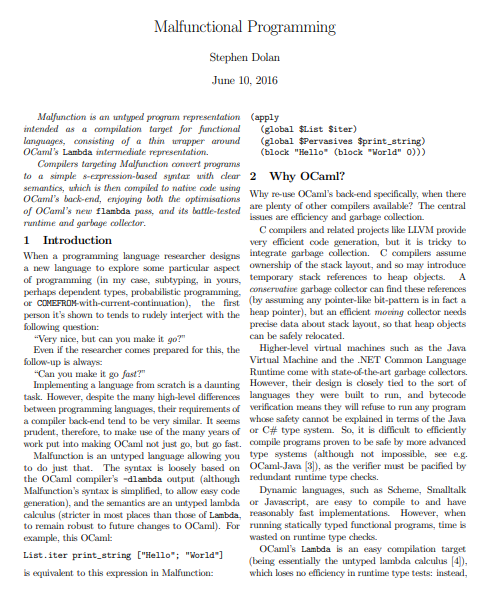
\includegraphics[width=.5\textwidth]{mlfpaper.png}
  \end{columns}
\end{frame}

\titlecard{A New OCaml backend for Idris}

\begin{frame}
  TODO:
  \begin{itemize}
    \item Idris has pluggable backends (C, JavaScript, PHP, ...)
    \item<2-> Sketch the pipeline (picture?)
    \item<3-> OCaml is a sensible target
    \item<4-> Dolan's malfunction backend is quite good
    \item<5-> But it compiles code after defunctionalisation
    \item<6-> We:
          \begin{itemize}
            \item Use OCaml's closures
            \item Compile nullary constructors to integers
          \end{itemize}
    \item<7-> Challenges
    \item<8-> Benchmark
  \end{itemize}
\end{frame}

\begin{frame}
  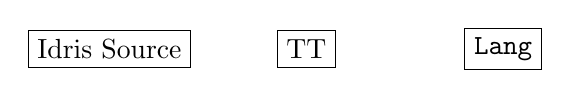
\begin{tikzpicture}
    \path
    ( 0,0) node [shape=rectangle,draw] {Idris Source}
    ( 2.5,0) node [shape=rectangle,draw] {TT}
    ( 5,0) node [shape=rectangle,draw] {\texttt{Lang}};
  \end{tikzpicture}
\end{frame}

\titlecard{An FFI between Idris and OCaml}

\begin{frame}
  Goal : to seamlessly use OCaml libraries from OCaml
\end{frame}

\begin{frame}[t]
  \frametitle{Representing OCaml types in Idris}

  \begin{displaymath}
    \begin{array}{@{}l}
      \textbf{data}\;\mathrm{OCaml\_Type} : \mathrm{Type} \to \mathrm{Type}\;\textbf{where} \\
      \quad
      \begin{array}{@{}l@{\quad:\quad}l}
        \mathsf{OCaml\_Str}   & \mathrm{OCaml\_Types}\;\mathrm{String} \\
        \mathsf{OCaml\_Float} & \mathrm{OCaml\_Types}\;\mathrm{Double} \\
        \mathsf{OCaml\_Bool}  & \mathrm{OCaml\_Types}\;\mathrm{Bool}   \\
        \mathsf{OCaml\_Unit}  & \mathrm{OCaml\_Types}\;()              \\
      \end{array}
    \end{array}
  \end{displaymath}

\end{frame}

\begin{frame}
  Challenge 1: IO monad vs pervasive effects
\end{frame}

\begin{frame}
  Challenge 2: Modules
\end{frame}

\begin{frame}
  Challenge 3: Wrapping libraries (Lwt)
\end{frame}

\titlecard{Demo}

\begin{frame}
  Future work:
  \begin{itemize}
    \item Generation of wrapper code from \texttt{.mli} files
  \end{itemize}
\end{frame}

\end{document}
